%!TEX root = ../NCVC3.tex

\mysection{加工条件の設定}

\vspace*{1zh}
 旋盤用の条件ファイルで設定します.拡張子はncjとなります.
以下に旋盤加工特有の設定ダイアログを列挙します.
フライス加工と違って送り速度に単位がない箇所があります.
G98毎分送りかG99毎回転送りによって変わりますので適宜読み替えてください.
送り速度に小数点が付く場合は[表記]タブの[Fパラメータ表記]を[小数点]にしておくと良いでしょう.

%\begin{minipage}{0.5\textwidth}
%\begin{figure}[H]
%\centering
%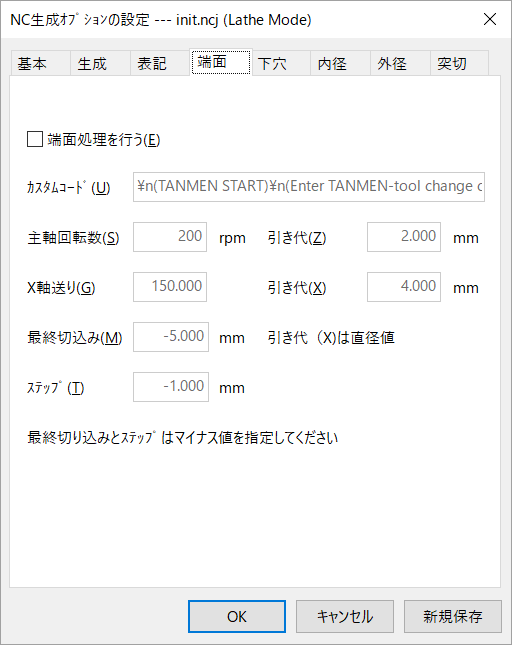
\includegraphics[scale=0.7]{No2/fig/ncj1.png}
%\caption{端面処理設定}
%\label{fig:ncj1.png}
%\end{figure}
%\end{minipage}
%\begin{minipage}{0.5\textwidth}
%\begin{figure}[H]
%\centering
%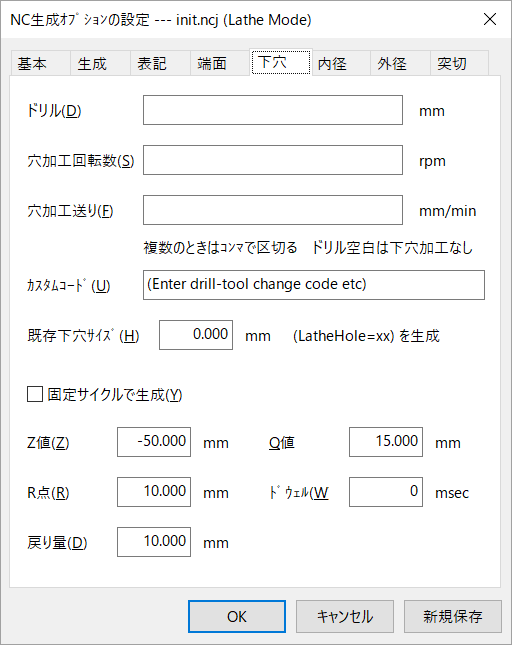
\includegraphics[scale=0.7]{No2/fig/ncj2.png}
%\caption{下穴加工設定}
%\label{fig:ncj2.png}
%\end{figure}
%\end{minipage}

%\begin{minipage}{0.5\textwidth}
%\begin{figure}[H]
%\centering
%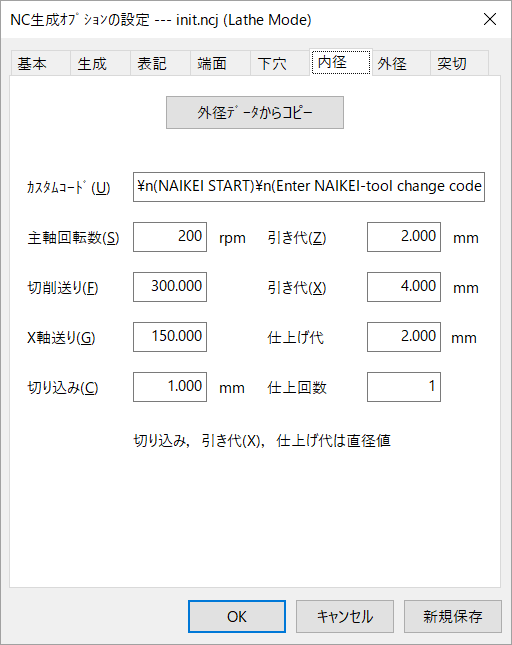
\includegraphics[scale=0.7]{No2/fig/ncj3.png}
%\caption{内径加工設定}
%\label{fig:ncj3.png}
%\end{figure}
%\end{minipage}
%\begin{minipage}{0.5\textwidth}
%\begin{figure}[H]
%\centering
%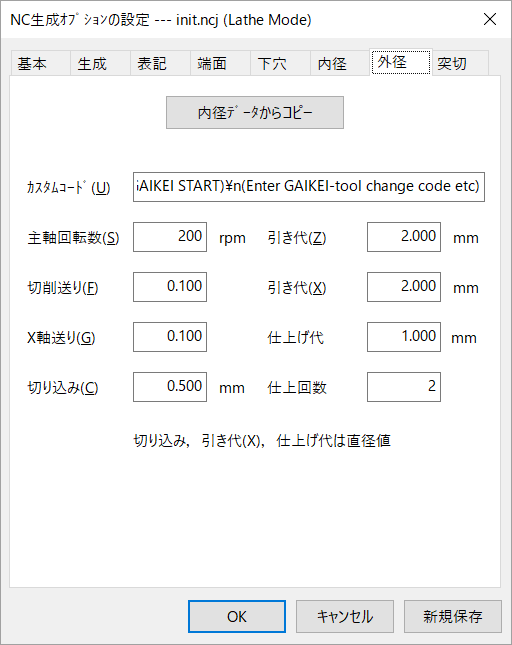
\includegraphics[scale=0.7]{No2/fig/ncj4.png}
%\caption{外径加工設定}
%\label{fig:ncj4.png}
%\end{figure}
%\end{minipage}

%\begin{figure}[H]
%\centering
%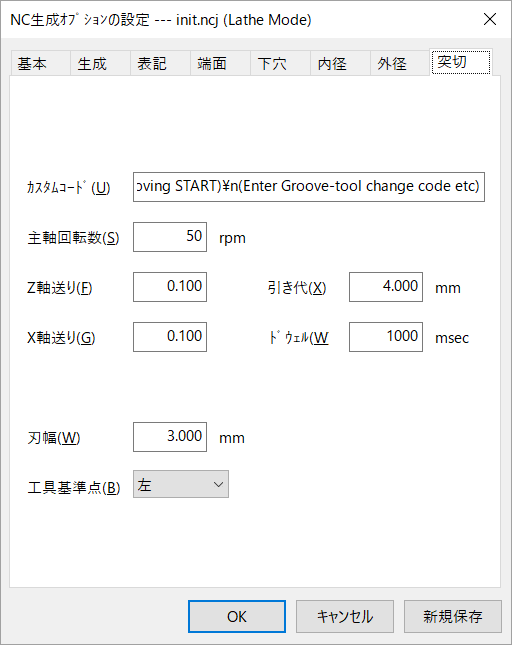
\includegraphics[scale=0.7]{No2/fig/ncj5.png}
%\caption{突切(溝)加工設定}
%\label{fig:ncj5.png}
%\end{figure}

\begin{itemize}
\item 端面\\
 端面処理を行いたい場合は[端面処理を行う]にチェックを入れてください.
[カスタムコード]には工具交換などのコードが挿入できます.``\,\yen{}n\,''で改行できるので複数行のブロックも挿入可能です.

\vspace*{1zh}
\item 下穴\\
 ドリルによる穴加工を行いたい場合は[ドリル]に使用するドリル径を入力してください.
空白の場合は下穴加工データを生成しません.複数のドリルを使用する場合はコンマで区切ります.
回転数と送り速度も同様にコンマで区切ります.中心にしか切削データを生成できません.
複合機のようなY軸移動はできません.汎用旋盤における芯押し台のイメージです.\\
 工具主軸回転などの特殊コード挿入には[カスタムコード]を利用してください.
端面処理と同様に``\,\yen{}n\,''で改行できます.\\
 被削材が加工前すでに中空の場合は[既存下穴サイズ]に入力してください.
生成データ中に(LatheHole=〇〇)のコメントが埋め込まれOpenGLソリッド表示の描画に反映されます.
[固定サイクルで生成]にチェックが入ると,G83固定サイクルモードで加工データが生成されます.\\
 ドリル切削か既存下穴サイズが無いと次の内径切削で図7のエラーが表示されます.

%\begin{figure}[H]
%\centering
%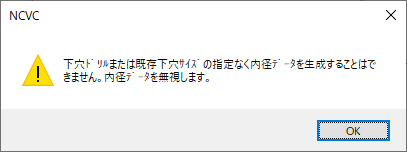
\includegraphics[scale=0.7]{No2/fig/error.png}
%\caption{内径生成時のエラー}
%\label{fig:error.png}
%\end{figure}

\vspace*{1zh}
\item 内径と外径\\
 荒取りと形状の仕上げ工程で切削データが生成されますが,荒取り工程では図8のように計算されます.
これの逆形状,つまり外径では右(端面に近い方)に太く左(主軸に近い方)に細い,内径では右に細く左に太い形状は,
荒取り工程の座標計算ができない場合があるのでご注意ください.
この場合は被削材を反対に取り付けるなど,切削工程の見直しが必要です.

%\begin{figure}[H]
%\centering
%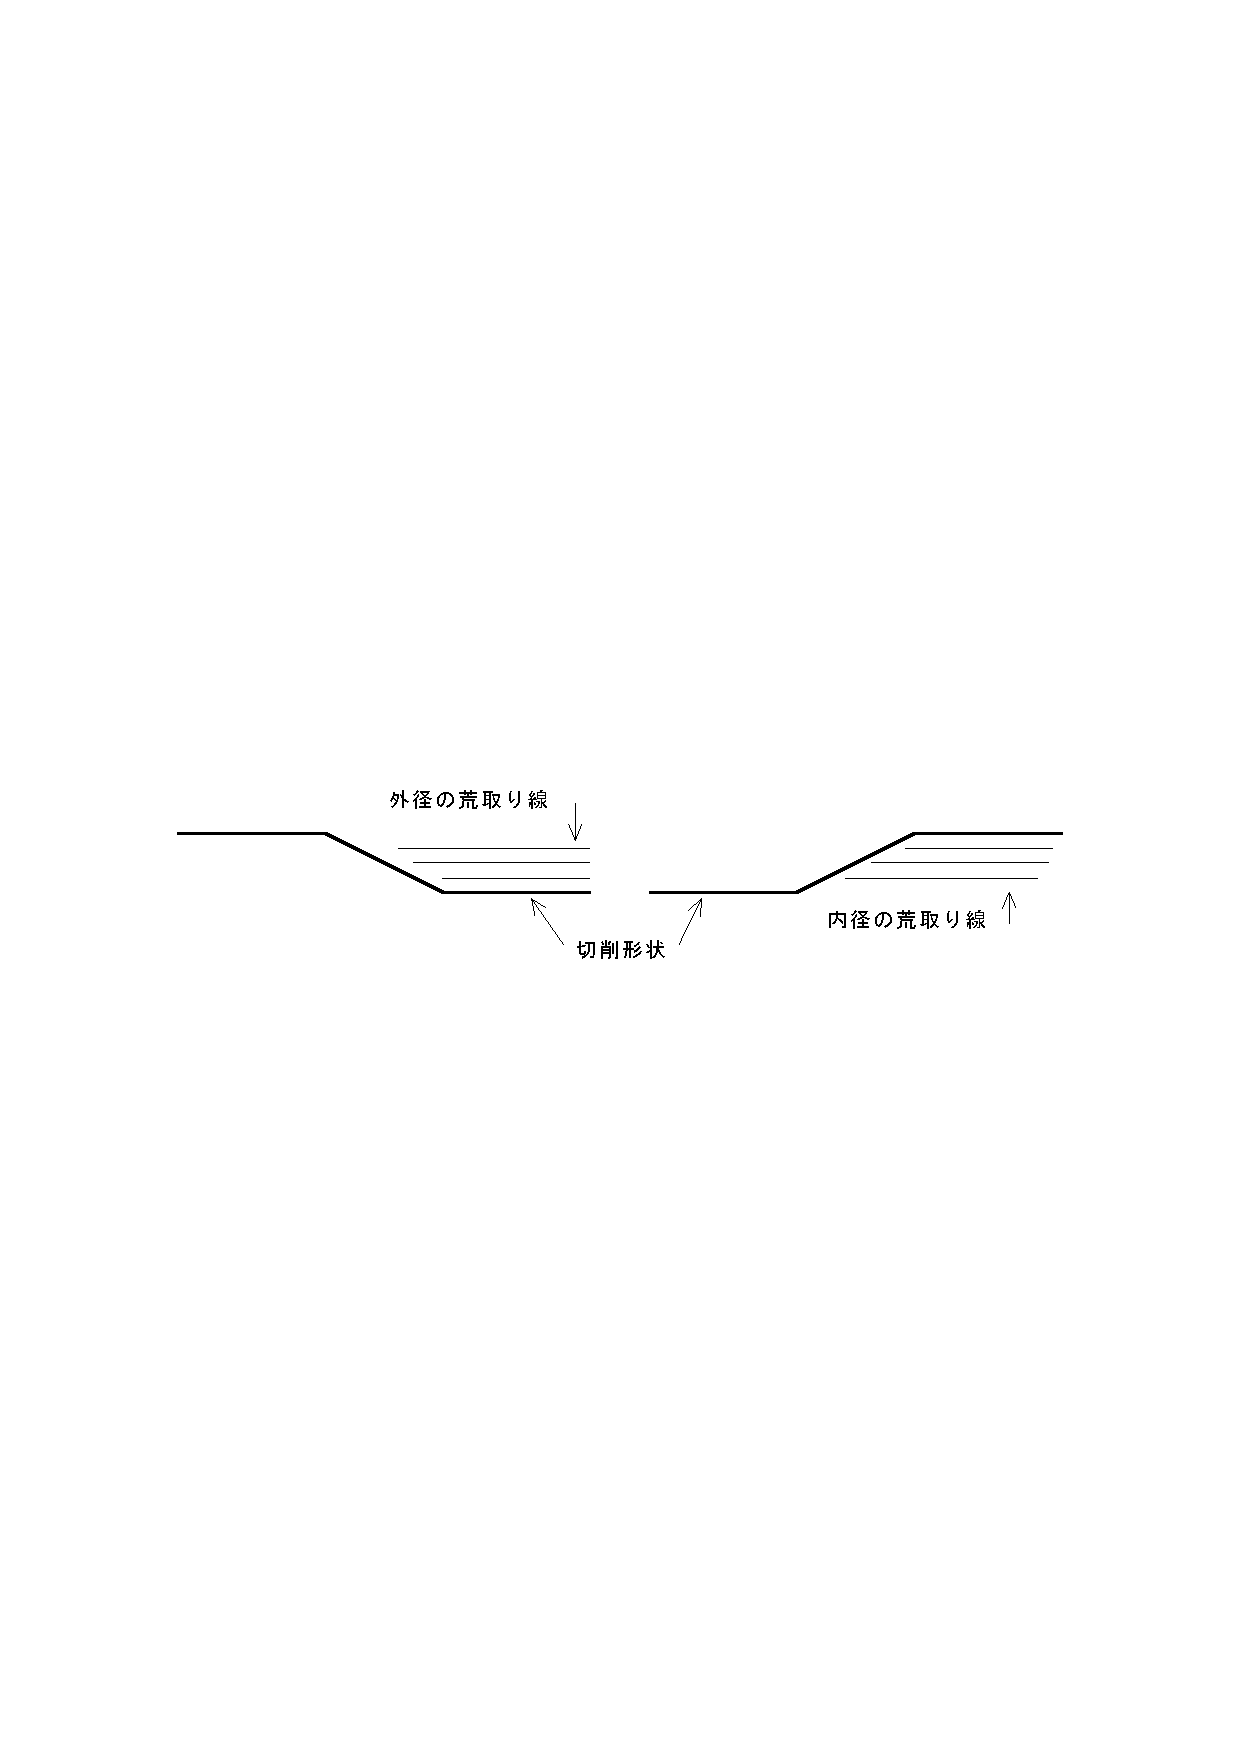
\includegraphics{No2/fig/inout.pdf}
%\caption{内外径の荒取り}
%\label{fig:inout.pdf}
%\end{figure}

\vspace*{1zh}
\item 突切\\
 作図した線の長さ(Z軸方向)が刃幅設定よりも長い場合と短い場合で生成される切削コードが違います.
図9のように長い場合はその線の長さ分だけZ軸方向の切削コードが生成されますが,短い場合はX軸方向を往復する切削コードが生成されます.
突っ切りバイトで前者の切削は仕上げ等で使うかもしれませんが,切り込み量などにご注意ください.通常後者になると思われます.

%\begin{minipage}{0.5\textwidth}
%\begin{figure}[H]
%\centering
%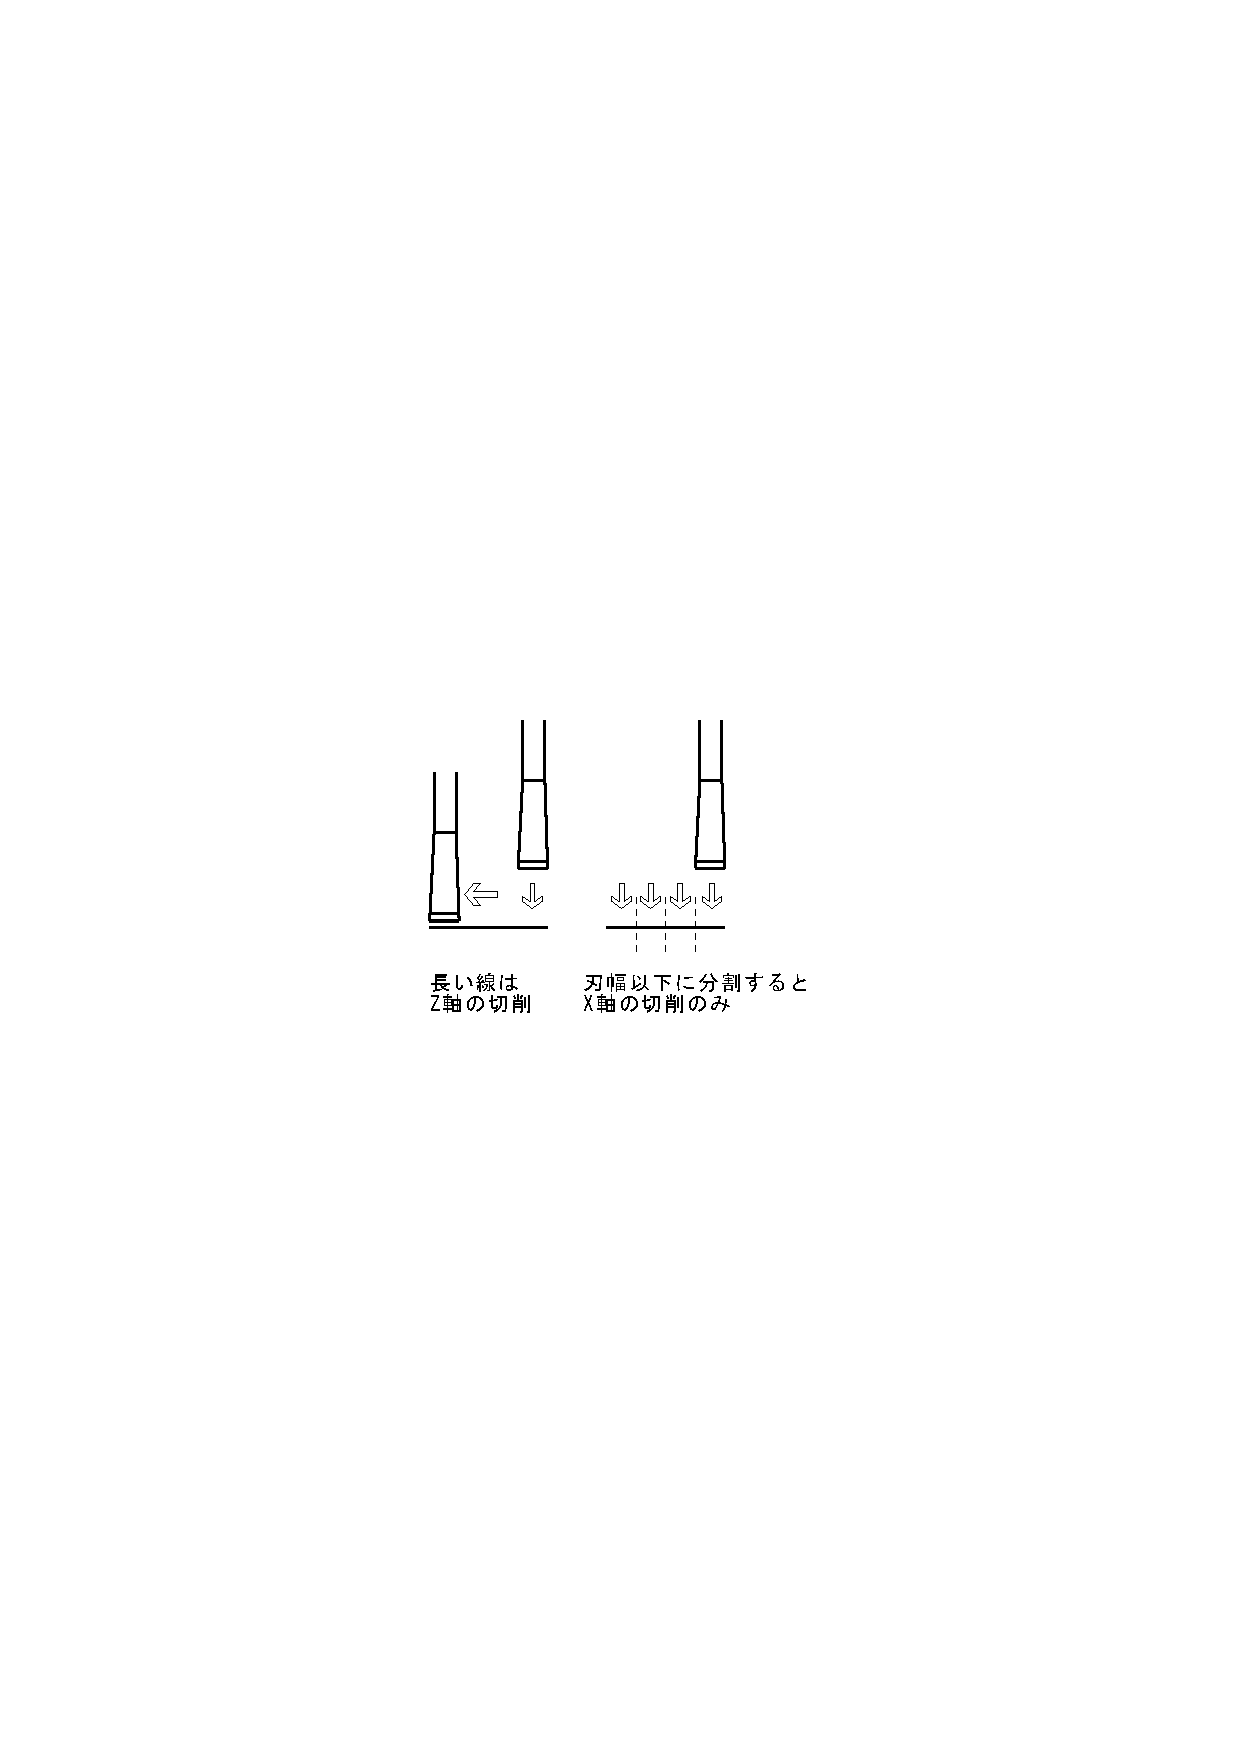
\includegraphics{No2/fig/groove1.pdf}
%\caption{作図線と切削コードの関係}
%\label{fig:ngroove1.pdf}
%\end{figure}
%\end{minipage}
%\begin{minipage}{0.5\textwidth}
%\begin{figure}[H]
%\centering
%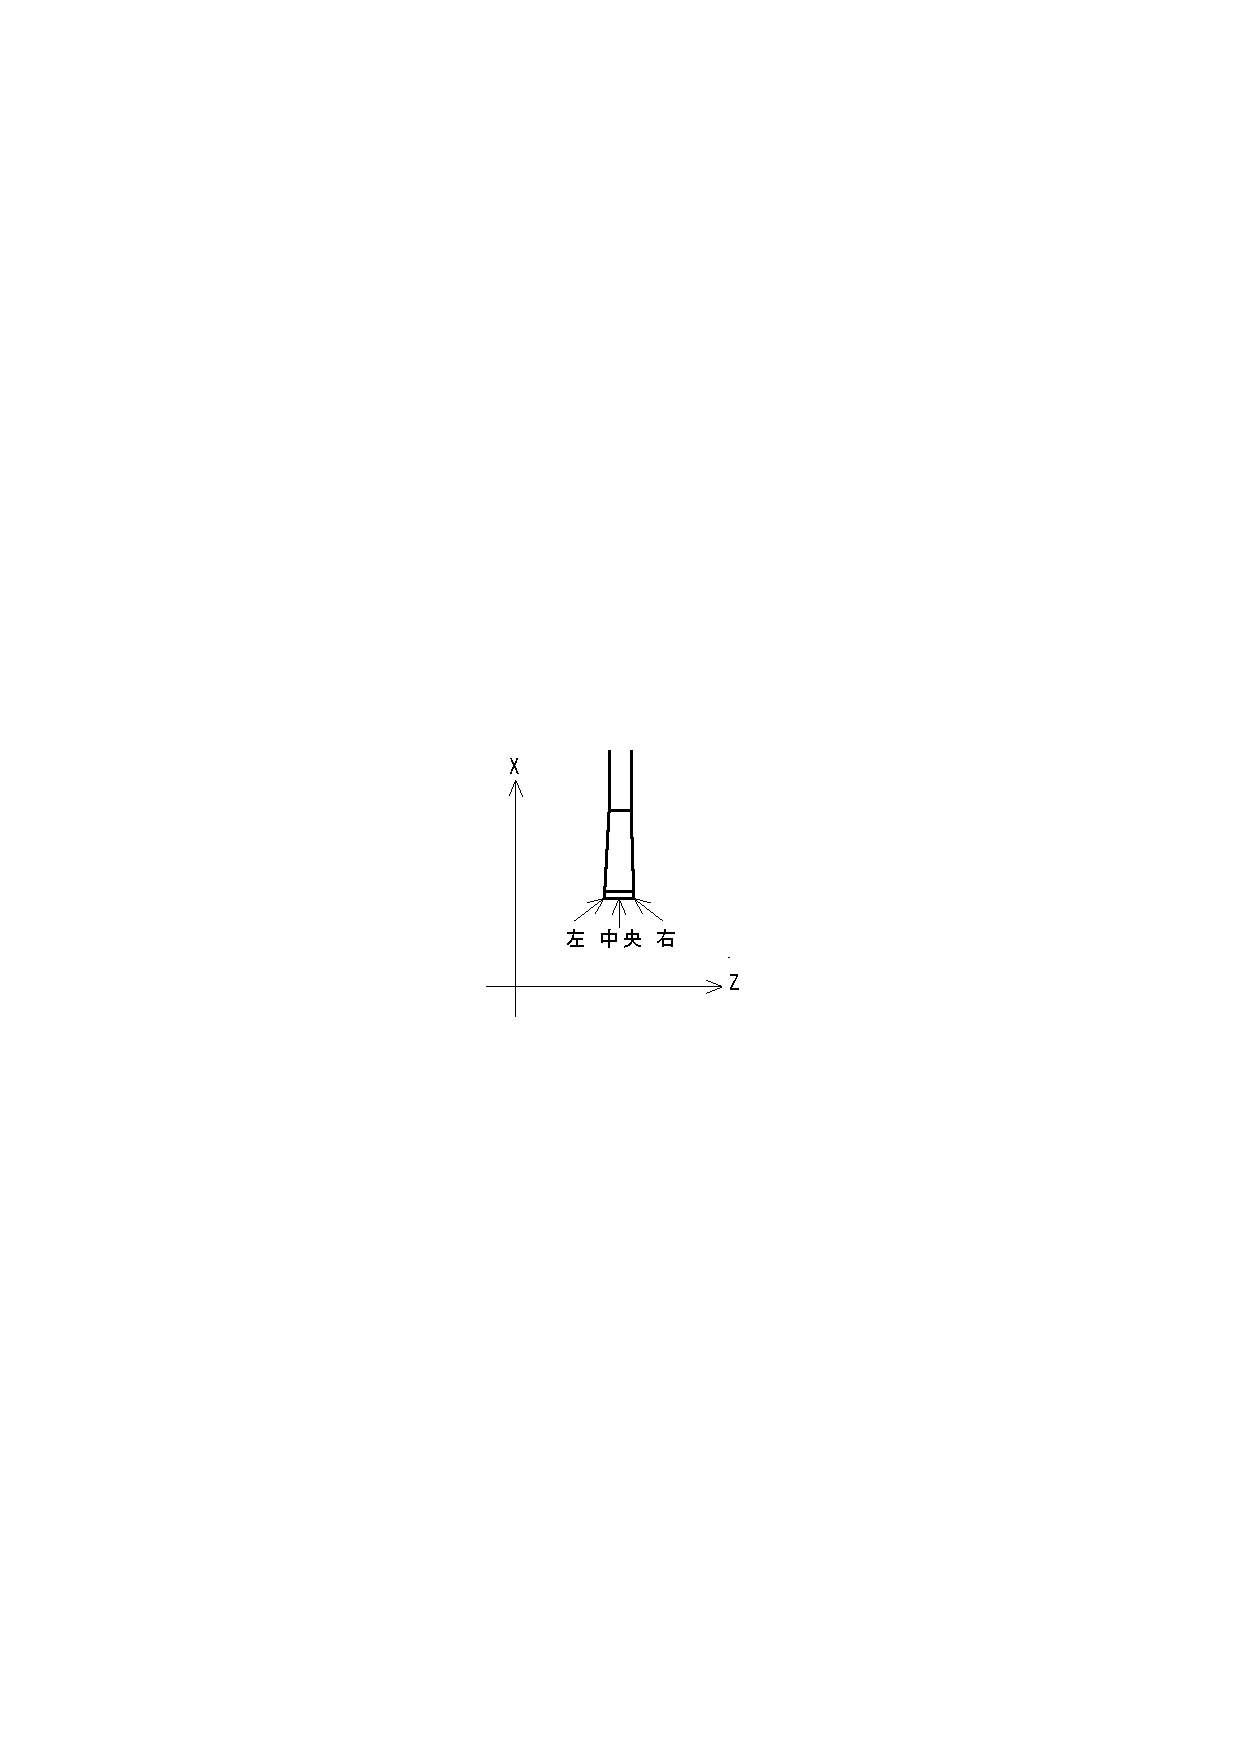
\includegraphics{No2/fig/groove2.pdf}
%\caption{工具基準点}
%\label{fig:groove2.pdf}
%\end{figure}
%\end{minipage}

 工具基準点は図10のようになっています.生成される座標が作図した線の左・中央・右になります.
\end{itemize}

 サンプルのカスタムヘッダー・フッターをリスト1に示します.
章の冒頭で述べたように旋盤に必要なG99毎回点送りやG96周速一定制御指示などを追加してください.
さらにカスタムヘッダー・フッターで使用可能な旋盤生成に関する置換キーワードを表1に示します.

\begin{minipage}[t]{0.75\textwidth}
\begin{lstlisting}[caption=Header.txt,numbers=none,label=lst:header.txt]
%
{ProgNo}
({MakeDate} {MakeTime})
({MakeUser} MADE {MakeNCD} FROM {MakeDXF} AND {MakeCondition})
(LatheView={LatheDiameter},{LatheZmax},{LatheZmin})
(ToolPos={ToolPosX},,{ToolPosZ})
{G90orG91}G54G99
M8
G96{Spindle}M3
\end{lstlisting}
\end{minipage}
\begin{minipage}[t]{0.25\textwidth}
\begin{lstlisting}[caption=Footer.txt,numbers=none,label=lst:footer.txt]
M9
M5
M30
%
\end{lstlisting}
\end{minipage}

\begin{table}[H]
\centering
\begin{tabular}{|p{3cm}|p{10cm}|}
\hline
ProgNo & 加工条件の[生成]タブにあるプログラム番号に置換 \\ \hline
LatheDiameter & 端面を示す線の一番下からY方向の距離×2に置換(被削材直径)\\ \hline
LatheZmax & 被削材を表す線の(ワーク座標原点をゼロとした)一番右座標 \\ \hline
LatheZmin & 被削材を表す線の(ワーク座標原点をゼロとした)一番左座標 \\ \hline
ToolPosX & 工具初期位置のY座標値(X軸相当)\\ \hline
ToolPosZ & 工具初期位置のX座標値(Z軸相当)\\ \hline
\end{tabular}
\end{table}
